% EUROPAR PAPER

\documentclass{llncs}
\usepackage{array}
\usepackage{multirow}

\usepackage{listings}
\usepackage[linesnumbered,ruled,vlined]{algorithm2e}

\usepackage{color}
\usepackage{tikz}
\usepackage{url}

\usepackage{fixme}
\fxsetup{status=draft,theme=color}

\usepackage{graphicx}

\usepackage{caption}
\usepackage{subcaption}
\captionsetup{compatibility=false}

\usepackage[babel=true]{csquotes}

\definecolor{dkgreen}{rgb}{0,0.6,0}
\definecolor{gray}{rgb}{0.5,0.5,0.5}
\definecolor{mauve}{rgb}{0.58,0,0.82}

\lstset{
		breaklines			= true
		, language			= C++
		, tabsize			= 4
		, captionpos			= b
		, frame                         = lines
		, basicstyle		= \small\ttfamily
		, keywordstyle		= \color{blue}
		, commentstyle		= \color{dkgreen}
		, stringstyle		= \color{red}
		, identifierstyle	= \ttfamily
		, columns		= flexible
	}

\begin{document}

\title{Parallel GMRES with Futures and Promises}

\author{Antoine Tran Tan\inst{1} \and Bryce Adelstein-Lelbach\inst{2} \and Joel Falcou\inst{1} \and Hartmut Kaiser\inst{2} \and
Daniel Etiemble\inst{1} }
\institute{LRI, Universit\'e Paris-Sud XI - Orsay, France \and CCT, Louisiana State University - Baton Rouge, USA}

\maketitle

\begin{abstract}
The exponential growth of available FLOPS requires the development of more sophisticated programming tools enabling significantly improved 
application efficiency and scalability on current and future architectures. We investigate the new execution model ParalleX \cite{ParalleX}, which defines a work queue based, message driven, fine grain parallelization scheme based on a global address space for highly asynchronous calculations. This paper uses HPX \cite{ParalleX}, a C++ library implementing the ParalleX execution model, to realize the GMRES operation from BLAS \cite{GMRES}. \emph{Futures}, a mechanism of asynchrony \cite{Futures1} \cite{Futures2} supported by ParalleX, are used to expose parallelism in our implementation. We examine the performance of this new HPX GMRES code, relative to conventional parallel GMRES implementations. 
\end{abstract}

\keywords{C++, Futures, Parallel Programming, High Performance Computing}

\section{Introduction}\label{Introduction}
High Performance Computing (HPC) is taking a new direction due to challenges provided by multicore and large scale systems. Indeed, the announced emergence of thousand billion core computers will significantly increases parallelism. The aim, therefore, will be no longer to make faster programs but to make programs that efficiently scale.\smallskip 

Clusters of multicore processors which are systems commonly used in HPC, use two programming models: shared memory model for SMP nodes and message passing model for the whole cluster. But using these models, parallel programs tend to follow the same programming rule consisting in implementing global barriers. ANL (Argonne National Laboratory) noticed the critical cost of barriers because
of latencies, system noises and non-uniform workloads especially in massively parallel machines. \cite{Barrier}\smallskip 

To solve this problem, the idea is to integrate asynchrony, a concept already existing in MPI but still difficult to implement. This paper thus introduces new concepts by means of ParalleX model which get away from conventional parallel programming models allowing to maximize asynchrony in calculations.\smallskip

Section \ref{Futures} introduces \emph{Futures} and \emph{Promises} mechanism in more general context. Section \ref{HPX} describes the High Performance ParalleX (HPX) runtime system \cite{ParalleX}, an experimental implementation of ParalleX. Section \ref{GMRES} defines the Generalized Minimal Residual algorithm (GMRES) \cite{GMRES} and discusses the results of its HPX implementation.

\section{Futures and Promises}\label{Futures}
Parallel programming models currently provide different ways to protect data shared between multiple threads (mutual exclusions, global barrier). But sometimes, the requirement is not necessarily to protect data but to simply synchronize concurrent operations encapsulated in different threads. One example is a thread which needs to wait that another thread finishes its work before running itself. To address this demand, object oriented programming research have proposed an alternative so called \emph{Futures} and \emph{Promises} \cite{Futures1} \cite{Futures2} which fully implements this concept.

\subsection{Definition}
In one hand, \emph{Futures} are objects encapsulating a value which will be available later. On the other hand, \emph{Promises} are objects intended to solve these \emph{Futures} using a function and some arguments. Programming with Futures is different from classical synchronous programming in the fact that tasks run in non-deterministic manner in time. Futures will then make it possible for applications to invoke asynchronous method without being interrupted. (cf. Figure \ref{thread})

\begin{figure}[h]
\begin{center}
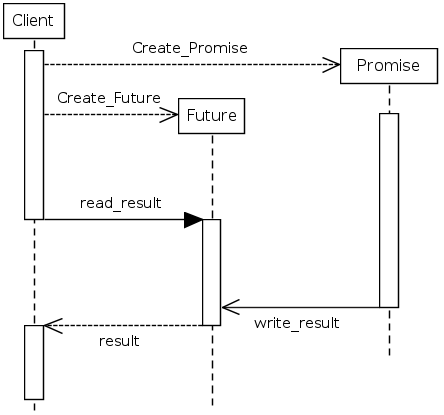
\includegraphics[scale=0.5]{Images/Im1.png}
\end{center}
\caption{Behavioural pattern of Futures and Promises}
\label{thread}
\end{figure}

\subsection{Example}
Here we illustrate the mechanism of Futures with an example. Suppose we want to
realize the following calculation:   
\begin{center}
  $y = f3(f1(a),f2(b))$
\end{center}

With sequential programming, the code could be written like:
\lstset{caption={Sequential C++ example code },label=example_future}
\begin{lstlisting}
  int a, b;
  int y1 = f1(a);
  int y2 = f2(b);
  y = f3(y1, y2);
\end{lstlisting}

With Futures programming, the code is written like:
\lstset{caption={C++ example code with Futures},label=example_future}
\begin{lstlisting}
  int a, b;
  future<int> y1 = async(f1,a);
  future<int> y2 = async(f2,b);
  y = f3(y1.get() , y2.get());
\end{lstlisting}


In this example (cf. Listing \ref{example_future}), Futures y1 and y2 each encapsulate one asynchronous function result. Required results are obtained by calling Futures \texttt{get()} method which lead to suspension of consumer threads until these results are available. The following timing diagrams illustrate the interest of Futures in terms of parallelism: with a syntax close to the sequential program, we had written a parallel code.

\begin{figure}[h]
      \begin{subfigure}[b]{0.5\textwidth}
	      \centering
	      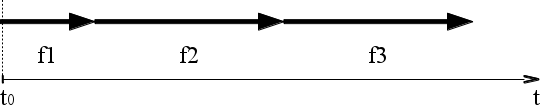
\includegraphics[scale=0.4]{Images/Im2.png}
	      \caption{Sequential program}
	      
      \end{subfigure}
      \begin{subfigure}[b]{0.5\textwidth}
	      \centering
	      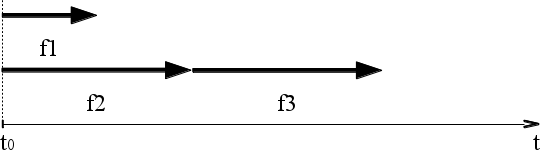
\includegraphics[scale=0.4]{Images/Im3.png}
	      \caption{Program with Futures}
      \end{subfigure}\\
      
      \caption{Timing diagrams of example code}
      \label{chronofuture}
\end{figure}

\subsection{Implementations}
The various implementations of Futures/Promises model are either directly integrated in languages (Alice ML, Scala) or integrated in specific libraries (OCaml, Java). A class implementation is also integrated in the last C++ standard \cite{Futuresc++}. From this point, Stellar group (Systems Technologies, Emergent Parallelism and Algorithms Research) of CCT (Center for Computation and Technology - Louisiana State University) has adapted this model in particular for distributed computing and grid computing. This adaptation, fully written in C++, consists of a runtime system named HPX (High Performance ParalleX). The next section will review the main elements of this system.   

\section{HPX Runtime System}\label{HPX}
HPX runtime system, designed by Stellar group, is an effective implementation of ParalleX paradigm that aims to increase performances by considering all obstacles encountered by conventional programming models. Thus, ParalleX combines several concepts that we will develop below.

\subsection{General Design}

\begin{figure}[h]
\begin{center}
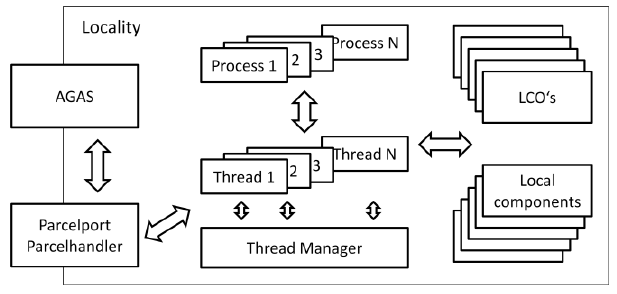
\includegraphics[scale=0.55]{Images/Im4.png}
\end{center}
\caption{Architecture of HPX runtime system}
\label{ArchiHPX}
\end{figure}

\subsubsection{AGAS - The Global Address Space}
A single adress space will open new perspectives like dynamic load balancing and dynamic graph related problems implementation. The PGAS model \cite{PGAS} partially solves this problem but don't allow objects to keep their name moving from a cluster node to another. Thus, Stellar group proposed a PGAS based model so called AGAS (Active Global Address Space) \cite{ParalleX} which assigns
global names (128 bits integers) to objects. While maintaining no coherence between cluster nodes, AGAS dynamically provides the correspondence between this global id and a local virtual address (LVA) \cite{ParalleX} which includes the node id, the type of the entity and its local memory address. This will help inter-node data migration.

\subsubsection{Parcels - Message Oriented Programming}
Message passing is an essential step when we work in a distributed memory. But the kind of message may vary with applications. On the one hand, we can move the data to the nodes which know in advance the work to accomplish; this is the solution of MPI. On the other hand, we can move the work to the nodes which already have their data; this is the solution of ParalleX. Thus, ParalleX incorporates the notion of \emph{Parcels} \cite{ParalleX} which are active messages including the destination address (provided by AGAS), the work to accomplish, some needed arguments and control elements for \emph{LCOs} that we will describe in section \ref{lcos}. This will enable dynamic resource
management and the use of distributed control flows.

\subsubsection{PX-threads - User Level Threads}
Thread migration between nodes is theoretically feasible but is still a costly operation in particular in heterogeneous parallel architectures. The preferred solution in ParalleX is to simply send requesting Parcels leading to the creation of a continuation thread in a certain locality. These continuation threads so called \emph{PX-threads} \cite{ParalleX} are user level threads, scheduled non-preemptively by a local thread manager (one per node) which knows in advance the corresponding node topology. This thread manager provides a PX-threads queue to each \emph{OS-thread} \cite{ParalleX} following the \enquote{first come first served} scheduling rule. Note that in conventional systems, an OS-thread is physically assigned to a processor core. Like a classical thread, a PX-thread may be in four different states which are: \emph{pending}, \emph{running}, \emph{suspended} and \emph{terminated}. The state of the PX-threads is controlled by the LCOs that we will describe below.

\subsubsection{LCOs - Thread Synchronisation Mechanism}\label{lcos}

\begin{figure}[h]
\begin{center}
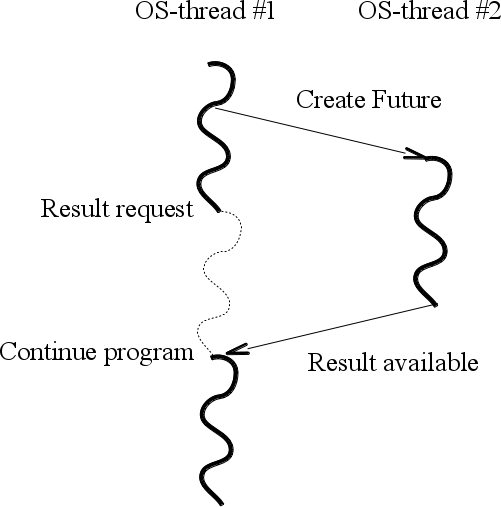
\includegraphics[scale=0.4]{Images/Im5.png}
\end{center}
\caption{Execution schematics of a Future in HPX}
\label{hpxthread}
\end{figure}

As we have seen in Section \ref{Introduction}, global barriers have become problematic. Thus, ParalleX integrates a lightweight thread synchronisation
mechanism in the form of \emph{LCOs} (Local Control Objects) \cite{ParalleX}. The LCOs are a class of objects which may locally create or reactivate (in a node) a PX-thread as a result of one or more events (ex: receipt of a Parcel). The LCOs may take several forms: \emph{semaphores}, \emph{mutexes}, \emph{Futures}. The Futures semantics described in section \ref{Futures} will thus enable event-driven thread creation, on-the-fly scheduling and effectively exploit the implicit parallelism of directed graph problems. Figure \ref{hpxthread} illustrates the use of Futures in the HPX system.

\section{GMRES Algorithm}\label{GMRES}
In the HPC field, linear systems resolution is increasingly done by iterative methods \cite{Methodes} (Jacobi, Gauss-Seidel, ...). These have indeed the advantage to provide high levels of parallelism in particular for large sparse systems: hence the idea to make an implementation of GMRES algorithm into HPX system. The GMRES method (Generalized Minimal Residual) \cite{GMRES} is an iterative algorithm solving the linear system $Ax=b$, where A is an invertible square matrix, from an initial guess $x_{0}$.\smallskip

At each iteration, this method calculates $x_{k} \in K_{k}$ where $K_{k}$ is a $k$-dimensional Krylov subspace, minimizing the Euclidian norm of the residual. But the amount of calculations and storage work increases whith the iteration. Thus, the algorithm is usually restarted every $m$ iterations using current approximate solution as initial guess before each restart step. ( GMRES(m) ) \cite{GMRES}

\subsection{The Gram-Shmidt Orthogonalization}
To reach this solution, we need to construct orthonormal vectors which constitute a Krylov space basis (Gram-Shmidt Orthogonalization) and then to perform several rotations to get a trivial system (upper triangular system). The main problem of GMRES is in the orthonormalization step. Indeed, the construction of each vector requires to realize two global communications: one during the orthogonalization step and the other during the normalization step.

\begin{algorithm}
\caption{GMRES Algorithm}
$r_0 \gets b-Ax_0$\\  
$v_0 \gets r_0/\|r_0\|_2$\\ 
\For{$i\leftarrow 0$ \KwTo $m-1$}{
    $z\gets Av_i$\\
    $h_{j,i} \gets \langle z,v_j\rangle , j=0,...,i$\\
    $\tilde{v}_{i+1} \gets z - \sum_{j=1}^{i}h_{j,i}v_j$\\
    $h_{i+1,i} \gets \|\tilde{v}_{i+1}\|_2 $\\
    $v_{i+1}\gets\tilde{v}_{i+1}/h_{i+1,i}$\\
    \# Apply Givens rotation to $H_{:,i}$\\
  }
  $y_m \gets argmin\|(H_{m+1,m}y_m - \|r_0\|_2e_1)\|_2$\\
  $x \gets x_0 + V_my_m$
\end{algorithm}

A first solution, that we won't deal with in this paper, is to minimize the inter-processes communications by adding redundancy in calculations. This approach so called \enquote{communication-avoiding} \cite{CAGMRES} results to the CA-GMRES version of the algorithm. A second solution is to change the synchronization model in order to reduce the communication overhead; this is the solution that we will examine below.

\subsection{Implementation with Futures}
In this study, we started from the original algorithm \cite{GMRES} developed by Y. Saad and M.H. Shultz. In each iteration, four kinds of operations are performed: sparse matrix-vector product, dot product, vector addition and vector scale. The most naive way to parallelize these various operations is to slice matrices and vectors and to attribute each pieces to a process (cf. Figure \ref{pargmres}). With HPX, the idea is to invoke several Futures in each iteration so that to perform an asynchronous calculation by domain. The second step including Givens rotations is mostly sequential and spend lower time than orthonormalization step. Then, we didn't take care of its optimization knowing its little influence on the performances.

\begin{figure}[h]
\begin{center}
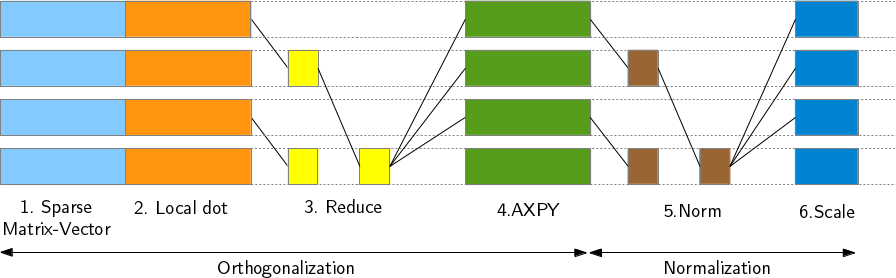
\includegraphics[scale=0.5]{Images/Im6.png}
\end{center}
\caption{Classical parallelization of GMRES}
\label{pargmres}
\end{figure}

\subsection{Experimental results}
This Section confronts the performances of HPX GMRES implementation with the one provided by PETSC \cite{Petsc}. Recognized as a reference in HPC field, PETSC performs its parallel calculations using MPI. These performance tests have been done for 5 problems from Matrix Market Collection and using the same initial guess $x_{0}$ and right-hand side vector $b$. We fixed the restart parameter to 30 to keep reasonable storage (Krylov basis vectors) and the maximum number of iterations to 1000, just enough for problems at hand. The used machine was a 2*6 core NUMA node. At this time, despite the popularity of this architecture and existing tools to manage it, HPX doesn't take care in giving NUMA domain affinity to PX-thread. This could be problematic when applications are memory bound: this is the case for GMRES when it uses BLAS interface. We will see below the impact on the performances.\smallskip  

To make a quantitative evaluation of performances, we used the Karp-Flatt metric: a parallelism measuring instrument developed from Amdahl's law and giving more informations about parallelism cost. The Karp-Flatt formula is:

\begin{eqnarray}
\alpha(p) &=&\frac{1/\gamma(p) - 1/p}{1-1/p} \label{KarpFlatt}
\end{eqnarray}
with\\
$\gamma$: Speedup of parallelism\\
$p$: Number of processors (or cores)\\

The major interest of this metric is to be representative of the evolution of parallelism cost. If $\alpha(p)$ increases with $p$, the declining efficiency of an algorithm is due to parallelism cost. If not, this is due to sequential part of the algorithm.\smallskip

Globally, HPX and Petsc codes scale relatively well while used cores are located in the same NUMA domain (from 1 to 6 cores). But when we use more cores (from 7 to 12), performances degrade because of inter-domain data exchange. We can notice that this degradation is worst for HPX because all data are located in the same NUMA domain. The distributed nature of Petsc code in which every core owns their data makes its scalability less impaired. From here, we'll restrict our focus on one NUMA domain (from 1 to 6 threads).\smallskip   

Figures \ref{add20} and \ref{orsreg_1} show performances for less sparse systems. In this case, each thread owns sufficient data to confer some scalability. Although execution times are equivalent, Karp-Flatt measuring show clearly that communication overhead has a more negative impact in HPX than in Petsc. Looking beyond the code structure, classical GMRES is largely synchronous and so it remains difficult to gain performance with asynchronism.\smallskip

Figure  \ref{pde900} show performances for very sparse systems. The sequential time is therefore smaller than others and so the overhead treshold appears clearly seeing HPX results. Here, the SpMV step scales less because of overlap of calculation by communications (starting from 4 threads). This overhead treshold is approximatively $25*10^{6}$ cycles with $2.4$ Ghz frequency.

\begin{figure}[h!]
\begin{center}
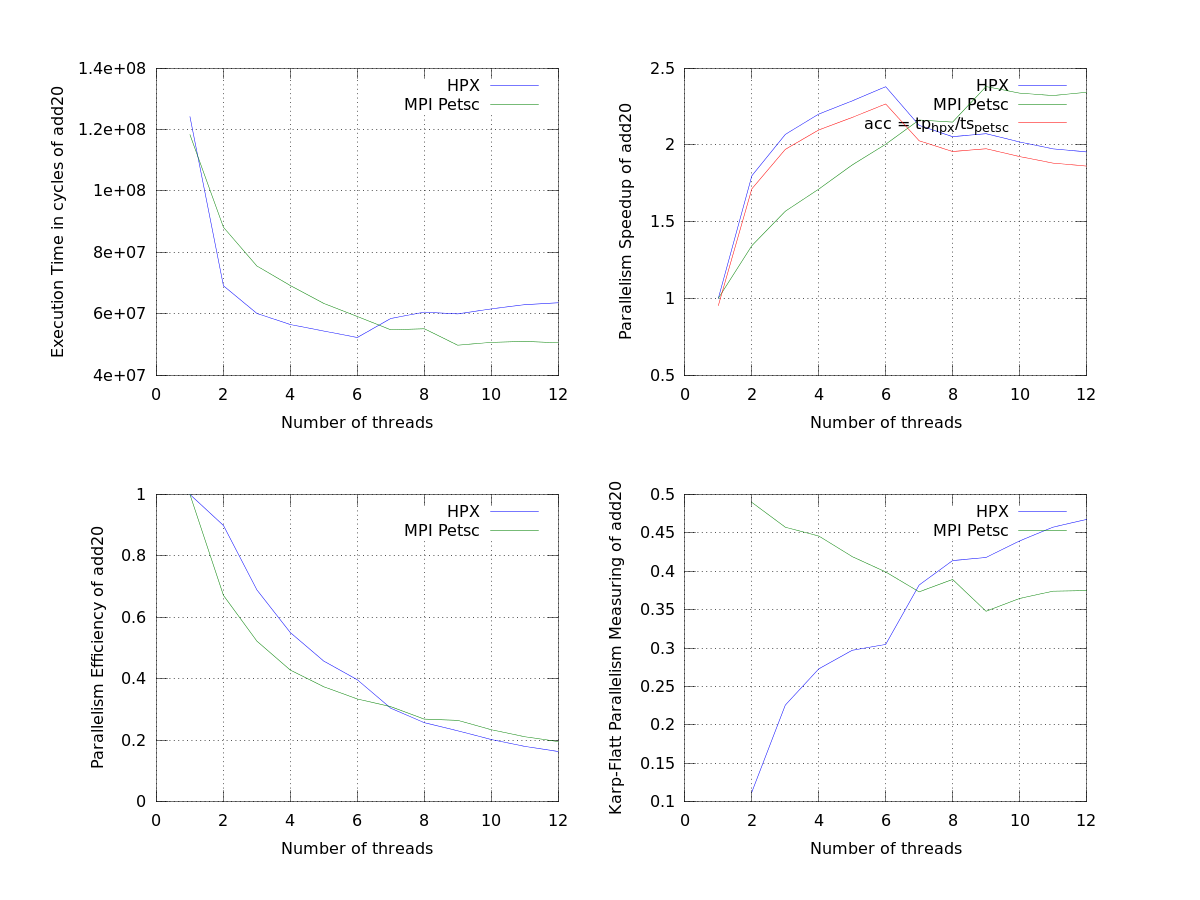
\includegraphics[scale=0.25]{Images/add20.png}
\end{center}
\caption{Performance measures of add20 ($2395\times2395$, 17319 entries)}
\label{add20}
\end{figure}

\begin{figure}[h!]
\begin{center}
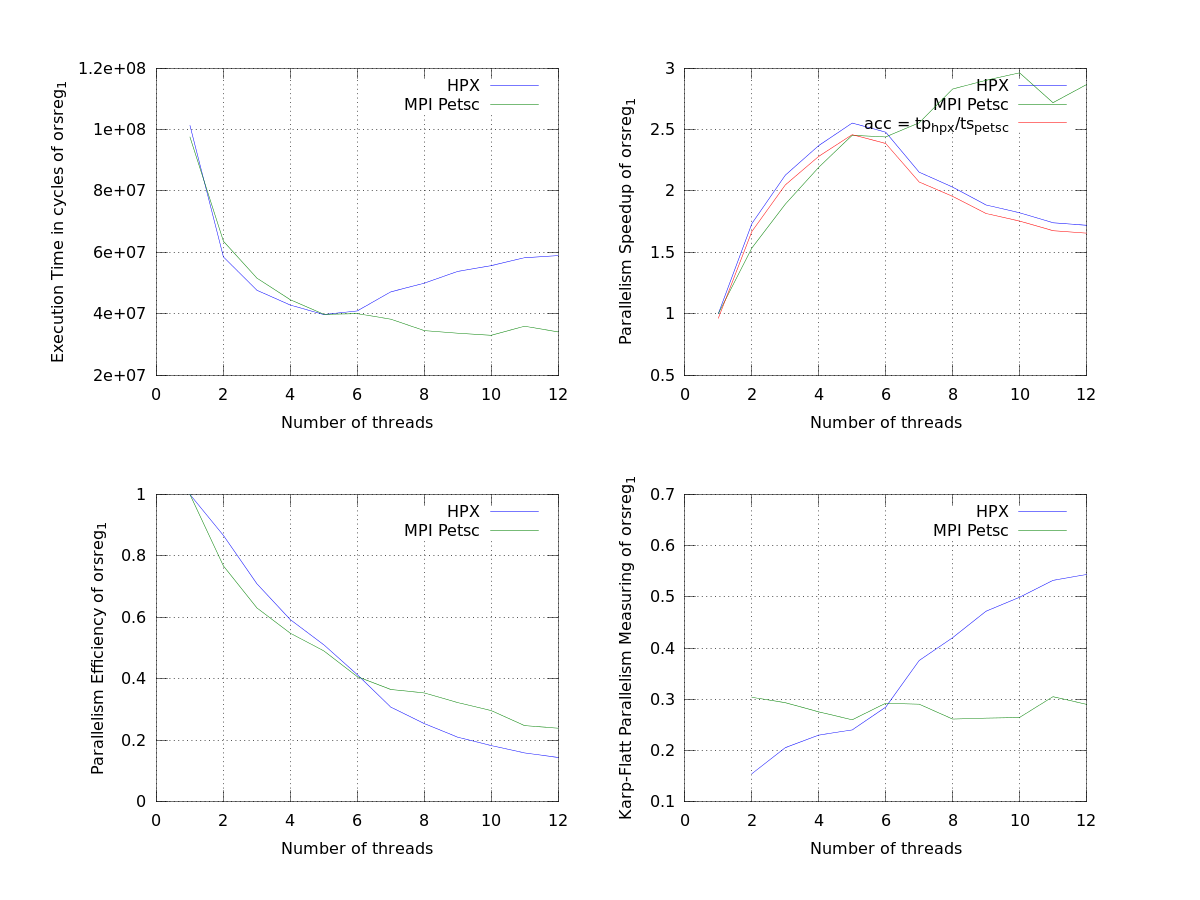
\includegraphics[scale=0.25]{Images/orsreg1.png}
\end{center}
\caption{Performance measures of orsreg$_1$ ($2205\times2205$, 14133 entries)}
\label{orsreg_1}
\end{figure}

\begin{figure}[h!]
\begin{center}
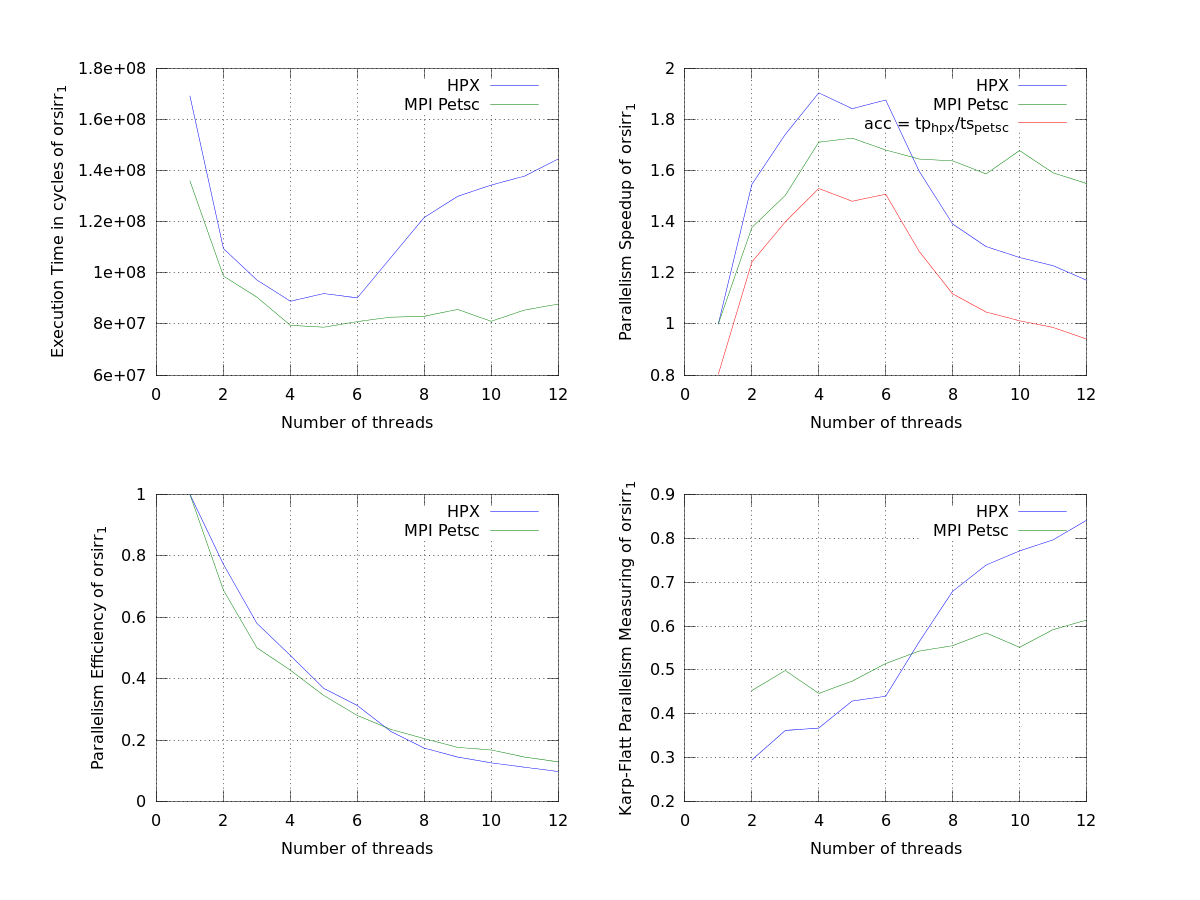
\includegraphics[scale=0.25]{Images/orsirr1.png}
\end{center}
\caption{Performance measures of orsirr$_1$ ($1030\times1030$, 6858 entries)}
\label{orsirr_1}
\end{figure}

\begin{figure}[h!]
\begin{center}
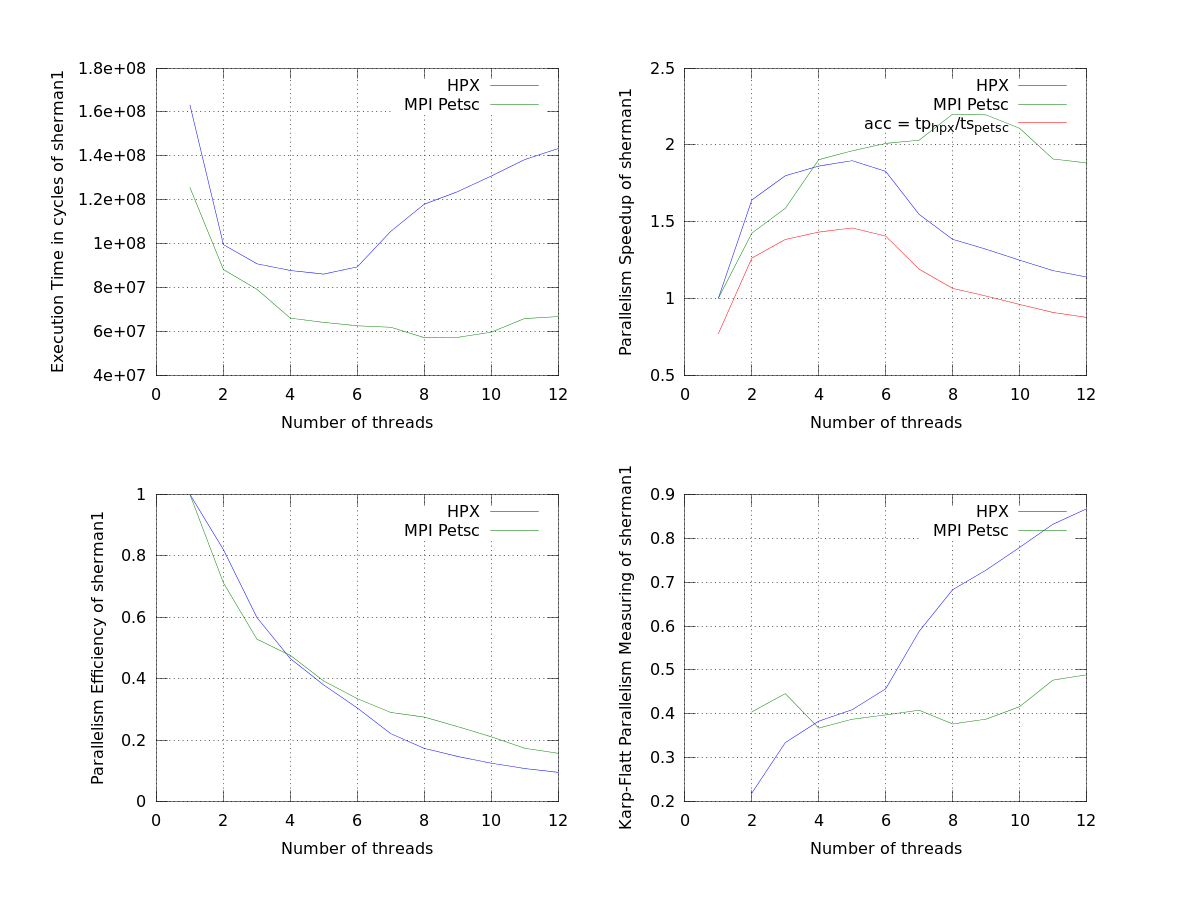
\includegraphics[scale=0.25]{Images/sherman1.png}
\end{center}
\caption{Performance measures of sherman$_1$ ($1000\times1000$, 3750 entries)}
\label{sherman1}
\end{figure}

\begin{figure}[h!]
\begin{center}
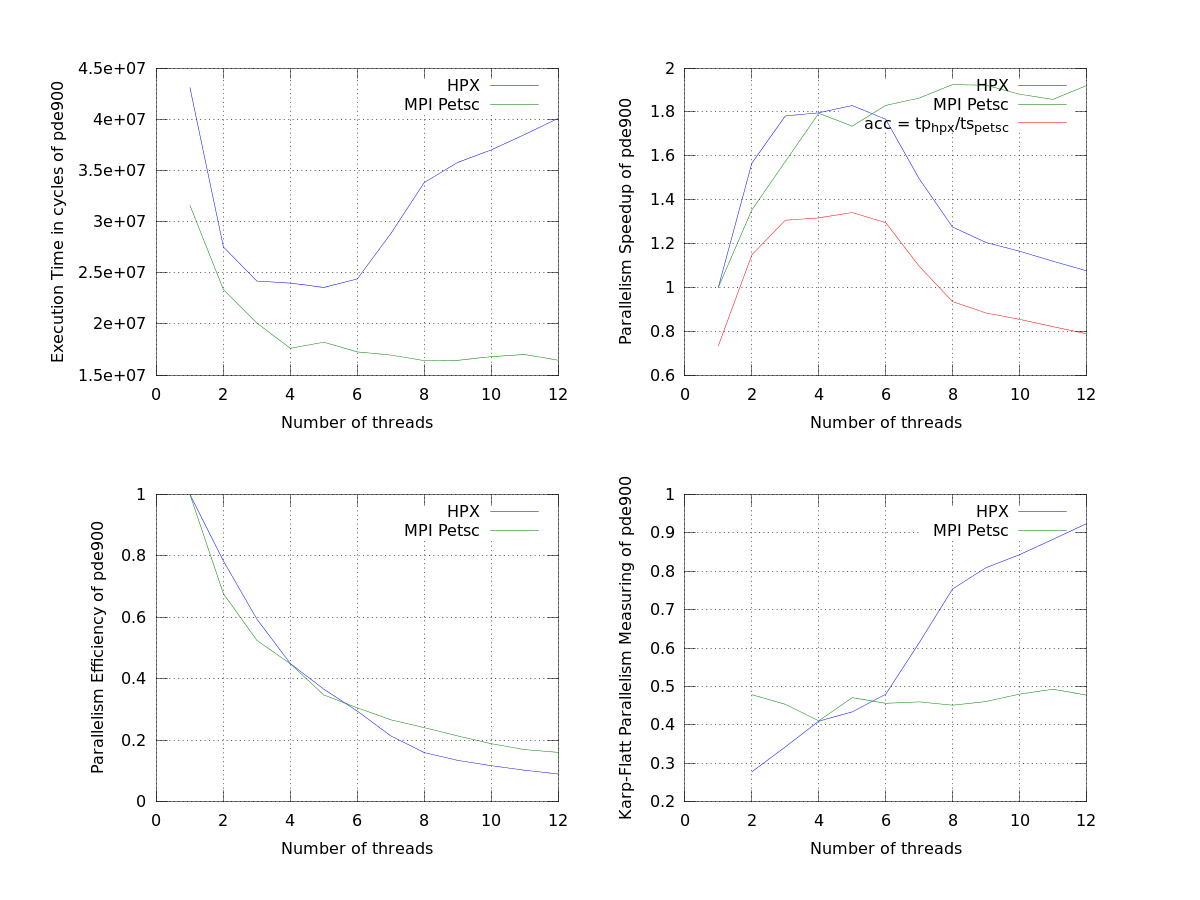
\includegraphics[scale=0.25]{Images/pde900.png}
\end{center}
\caption{Performance measures of pde900 ($900\times900$, 4390 entries)}
\label{pde900}
\end{figure}


\section{Conclusion}
Other versions of the algorithm exist like Pipelined GMRES (p(l)-GMRES) \cite{Parall_GMRES} in which some of calculation steps are interlaced with each other so that to hide global communications. This version integrating more asynchronous calculations could be investigated with HPX and compared to the actual Petsc implementation.

\bibliographystyle{abbrv}
\bibliography{main}

\end{document}
